\chapter{Pulse Shape and Learned Representations}

\section{Physics question and data scope}

The B-stack waveform has only 18 samples per readout channel, but those samples encode several
distinct effects: the prompt scintillation pulse, electronics shaping, baseline excursions,
late charge, saturation, and occasional malformed or overlapping pulses.  This chapter
summarises the studies that asked whether learned waveform representations expose useful
structure beyond transparent shape variables.  The emphasis is deliberately conservative:
learned embeddings are useful only if they survive the same run-held-out and leakage-sentinel
standards used elsewhere in the analysis.

The recurring raw-data gate is the S00 B-stave selection.  For a waveform $x_{e,c,s}$ from event
$e$, channel $c$, and sample $s$, the pedestal-subtracted pulse is
\begin{equation}
  y_{e,c,s} = x_{e,c,s} - {\rm median}\{x_{e,c,0},x_{e,c,1},x_{e,c,2},x_{e,c,3}\},
  \qquad A_{e,c} = \max_s y_{e,c,s}.
\end{equation}
The selected B-stack pulse table keeps the even B-stave channels B2, B4, B6, and B8 when
$A_{e,c}>1000$ ADC.  The full gate reproduces 640737 selected pulse records from raw ROOT in
the P01 and P09 studies before fitting any representation or anomaly model.  The P02 discovery
study reused the same gate on a 60000-pulse subset of runs 50 and 58--65.

\section{Traditional and learned representations}

The traditional representation is principal component analysis (PCA) of amplitude-normalised
waveforms, optionally augmented by hand-engineered shape summaries such as peak sample, area,
late fraction, width, plateau, asymmetry, and template residuals.  PCA provides the linear
rank-$k$ approximation
\begin{equation}
  \hat{z}_i^{\rm PCA}(k) = \bar{z} + U_k U_k^{T}(z_i-\bar{z}),
  \qquad
  {\cal L}_{\rm rec} = \frac{1}{18N}\sum_i \lVert z_i-\hat{z}_i\rVert_2^2 ,
\end{equation}
where $z_i$ is the normalised 18-sample pulse.  The learned comparator is a compact autoencoder,
either a plain fully connected autoencoder in the P02 discovery study or a masked-denoising
autoencoder in P01.  In the latter case, random samples are masked during training and the network
minimises the same reconstruction loss while learning a bottleneck representation
\begin{equation}
  h_i=f_\theta(z_i), \qquad \hat{z}_i=g_\phi(h_i), \qquad
  \min_{\theta,\phi} \sum_i \lVert z_i-g_\phi(f_\theta(\tilde{z}_i))\rVert_2^2 .
\end{equation}

\begin{table}[H]
\centering
\caption{Representation benchmarks on held-out or discovery samples.  P01 intervals are
95\% run-block bootstrap CIs on held-out runs 42, 57, 64, and 65.  P02 is an unsupervised
60000-pulse discovery benchmark without a predictive run split; it is therefore used as
representation evidence, not as a downstream physics claim.}
\begin{tabular}{llrrrr}
\toprule
Study & Method & Latent dim. & Metric & Value & 95\% CI \\
\midrule
P01 & PCA & 4 & recon. MSE & 0.01337 & [0.00922, 0.01696] \\
P01 & masked AE & 4 & recon. MSE & 0.01428 & [0.01030, 0.01772] \\
P01 & hand-shape probe & -- & balanced acc. & 0.3527 & [0.3227, 0.3650] \\
P01 & AE-4 probe & 4 & balanced acc. & 0.3638 & [0.3446, 0.3707] \\
P02 & PCA & 2 & recon. MSE & 0.02622 & -- \\
P02 & AE & 2 & recon. MSE & 0.01294 & -- \\
P02 & PCA & 4 & recon. MSE & 0.00880 & -- \\
P02 & AE & 4 & recon. MSE & 0.00527 & -- \\
P02 & PCA & 8 & recon. MSE & 0.00166 & -- \\
P02 & AE & 8 & recon. MSE & 0.00292 & -- \\
\bottomrule
\end{tabular}
\end{table}

The resulting picture is not a simple ``ML wins'' statement.  At very low dimension the
nonlinear AE is clearly more compact in P02, improving reconstruction MSE by 50.6\% at
dimension 2, 40.6\% at dimension 3, and 40.1\% at dimension 4.  At dimension 8, however, linear
PCA is already close to lossless for this detector waveform and beats the small AE.  P01's
strict run-held-out benchmark reaches the same qualitative conclusion from the opposite
direction: the masked AE is a useful compact nonlinear embedding, but PCA and hand-shaped
features remain strong baselines.  The downstream stave probe improves only from 0.3527 to
0.3638 balanced accuracy, and the interval overlap means it should not be read as a robust
physics win.

\begin{figure}[H]
\centering
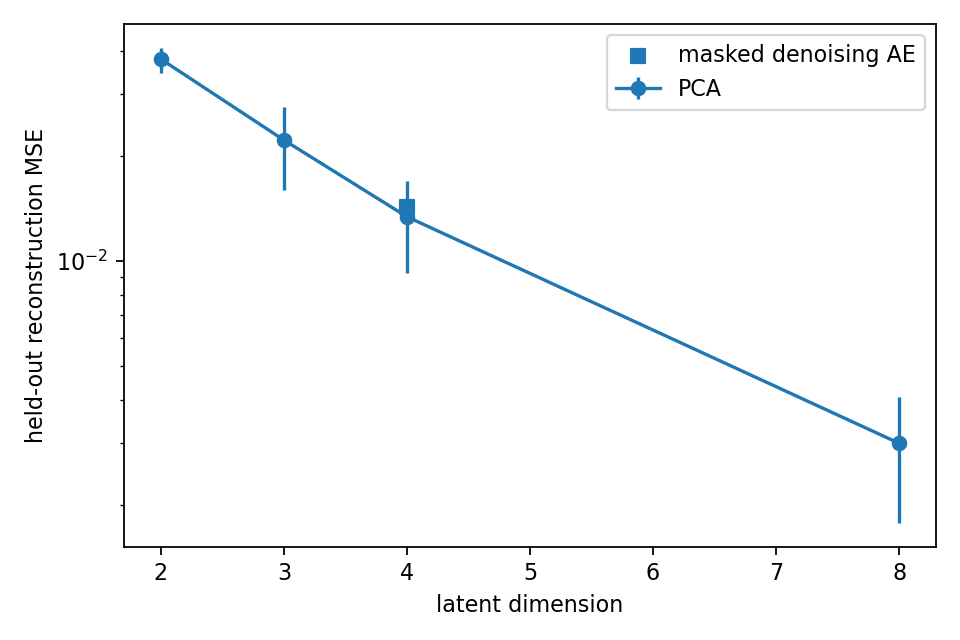
\includegraphics[width=0.92\textwidth]{../figures/reports/1780997954.15517.0cbc248c__p01_self_supervised_waveform_representation/fig_reconstruction_head_to_head.png}
\caption{P01 held-out reconstruction comparison between PCA and the masked-denoising
autoencoder.  The run-held-out split protects the reconstruction and probe summaries from
same-run leakage.}
\end{figure}

\begin{figure}[H]
\centering
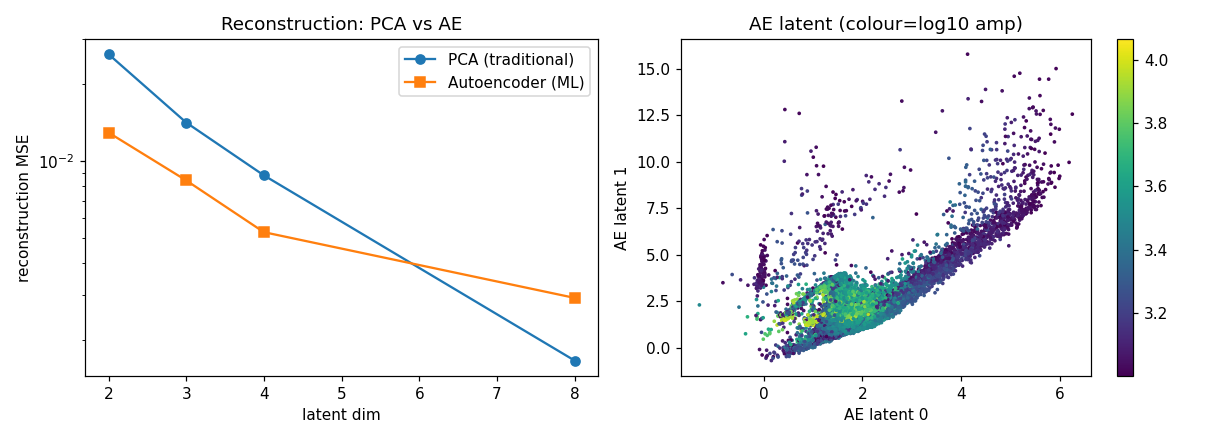
\includegraphics[width=0.92\textwidth]{../figures/reports/P02_pulse_representation_discovery/fig_pca_vs_ae_and_latent.png}
\caption{P02 compact-representation scan and latent map.  The AE is best at dimensions 2--4,
while PCA dominates once eight linear components are allowed.}
\end{figure}

\section{Unsupervised pulse types}

P02 used the AE latent space for label-free clustering.  The first eight PCA components already
explain 99.7\% of the waveform variance, but the low-dimensional AE map separates a small
morphology that is not obvious from amplitude alone.  K-means with five clusters on the AE-3
latent found two dominant normal pulse groups, peaking at samples 7--8, and an early-peak class
with peak sample near 3, low amplitude, and near-zero or pathological integrated area.  The
early-peak clusters account for about 2640 of 60000 pulses, or roughly 4.4\% of the discovery
sample.

\begin{table}[H]
\centering
\caption{P02 AE-cluster interpretation.  Counts are from the 60000-pulse discovery subset.}
\resizebox{\textwidth}{!}{%
\begin{tabular}{lrrrl}
\toprule
Cluster family & Clusters & Pulses & Median peak sample & Interpretation \\
\midrule
Normal, higher amplitude & 2 & 24201 & 7 & Ordinary late-positive pulse family \\
Normal, lower amplitude & 3 & 25137 & 8 & Ordinary lower-amplitude pulse family \\
Intermediate shape & 0 & 8025 & 5 & Mixed prompt/late morphology \\
Early-peak anomalous & 1, 4 & 2637 & 3 & Low-area early peak / pretrigger-like atom \\
\bottomrule
\end{tabular}
}
\end{table}

\begin{figure}[H]
\centering
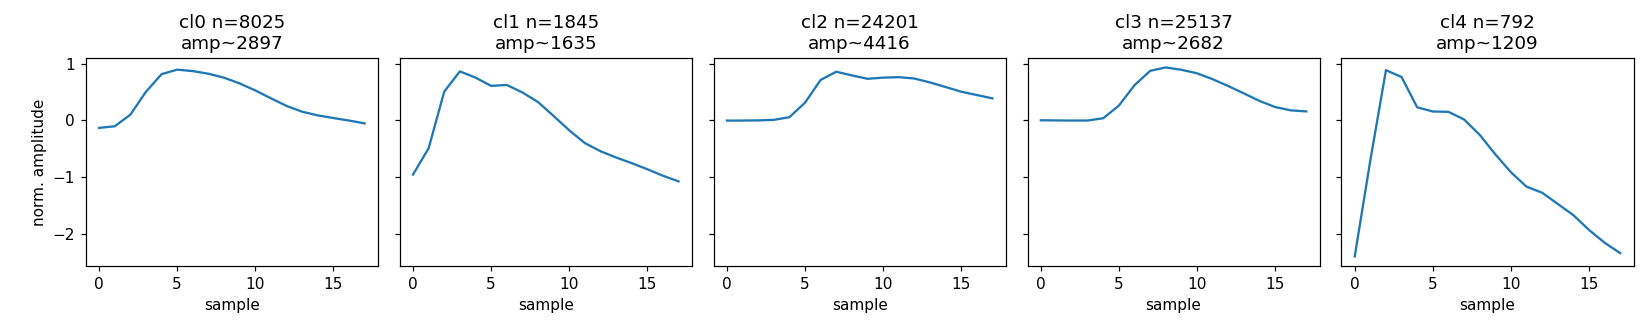
\includegraphics[width=0.92\textwidth]{../figures/reports/P02_pulse_representation_discovery/fig_cluster_mean_waveforms.png}
\caption{Mean waveforms for P02 latent clusters.  The early-peak family was found without
labels and motivated the later anomaly-taxonomy studies.}
\end{figure}

This is one of the strongest positive uses of representation learning in the pulse-shape
program: not a black-box classifier, but a hypothesis generator that exposes a coherent waveform
atom for later audits.  It also illustrates the limit of unsupervised evidence.  Cluster labels
are inferred from waveform morphology and cross-tabulations; they are not particle species,
pile-up truth, or timing truth.

\section{Rare waveform anomaly taxonomy}

P09 turned the P02 discovery into a held-out anomaly audit.  The traditional method ranked
pulses by robust train-run template residuals and transparent shape scores, including
\texttt{q\_template}, peak sample, late fraction, baseline residual, saturation count,
duplicate-channel timing span, secondary peak, and undershoot.  The learned method combined PCA
reconstruction error, AE reconstruction error, and an IsolationForest density score in PCA+AE
latent space.  The gallery was balanced by held-out run and stave, while identifiers were
excluded from scoring features.

\begin{table}[H]
\centering
\caption{P09a top-128 anomaly gallery audit on held-out runs.  Intervals are 95\% bootstrap CIs
over held-out runs.}
\begin{tabular}{lrrr}
\toprule
Method & Curated precision & Novel precision & Duplicate-event rate \\
\midrule
Robust template ranker & 0.898 [0.852, 0.945] & 0.555 [0.508, 0.625] & 0.0156 [0, 0.0469] \\
PCA+AE+IsolationForest & 0.883 [0.797, 0.969] & 0.766 [0.703, 0.828] & 0.0469 [0, 0.0938] \\
Balanced random & 0.180 [0.125, 0.242] & 0.164 [0.109, 0.227] & 0.0166 [0, 0.0473] \\
\bottomrule
\end{tabular}
\end{table}

The traditional ranker has the slightly higher curated precision, while the learned ranker is
substantially better for novel taxa.  This is a useful and interpretable division of labour:
robust template scores are good at recovering known curated failures, whereas the latent-density
score is better at surfacing morphology that was not already encoded by the hand score.  The
dominant held-out taxa were unassigned common pulses (91.5\%), novel early-pretrigger pulses
(4.02\%), novel delayed peaks (2.65\%), baseline excursions (1.23\%), and a much smaller
broad-template-mismatch class (0.272\%).

P09c then asked whether delayed-peak and broad-template-mismatch taxa propagate into timing,
charge, baseline, or pile-up sentinels.  For the delayed-peak target, the learned latent-isolation
score separated the target stratum much more effectively than the frozen robust-template score
(average precision 0.789 versus 0.433).  The same target had a large pile-up-score displacement
of 14.66 with CI [14.60, 14.70], a charge-bias delta of -4.82 with CI [-4.95, -4.65], and no
timing-tail or baseline-excursion enrichment under the frozen definitions.  The broad-template
class had only 162 held-out targets and one veto-like positive, so its perfect recover-veto AP in
one ML row is explicitly low-evidence and not a robust operational result.

\section{Downstream value and leakage sentinels}

The strongest caveat is that a good latent space is not automatically a good physics observable.
P01c and P01e repeatedly tested whether AE latents improve downstream waveform probes after
stricter controls.  In P01c, residual hand/PCA features reached balanced accuracy 0.331
[0.304, 0.349] on a leakage-sentinel task, while residual AE-4 reached only 0.235
[0.221, 0.246].  The amplitude/topology proxy and target-topology leakage sentinel were much
larger than either representation, showing how easily a representation claim can be dominated by
detector topology rather than pulse shape.  In P01e's strict timing audit, traditional hand-shape
ridge and AE-latent ridge were effectively tied: $\sigma_{68}=1.962$ ns [1.882, 2.064] for the
traditional model and $\sigma_{68}=1.965$ ns [1.885, 2.058] for the AE latent.

\begin{figure}[H]
\centering
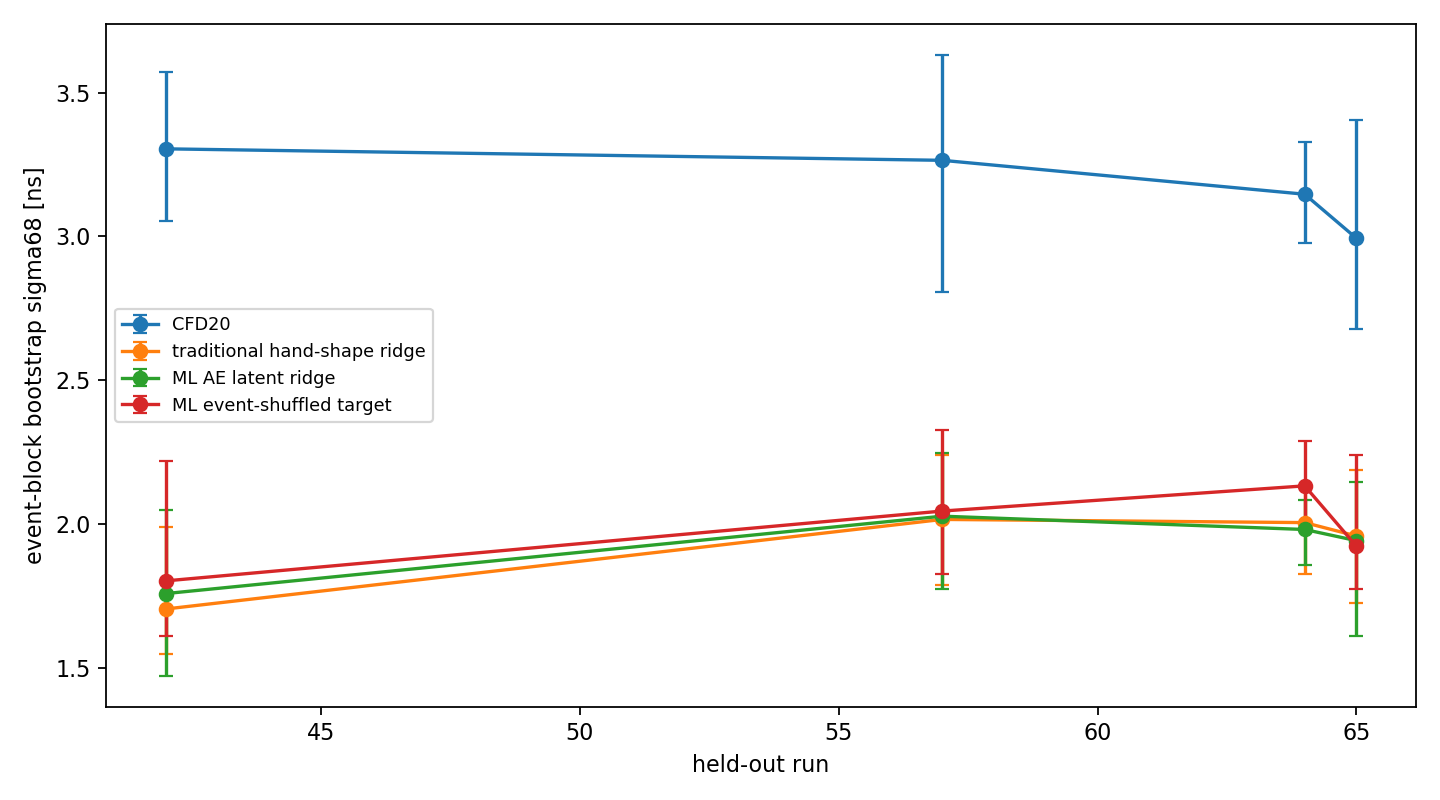
\includegraphics[width=0.86\textwidth]{../figures/reports/1781010798.1019.19c63d1a__p01e_strict_latent_timing_audit/fig_loro_sigma68.png}
\caption{P01e strict leave-one-run-out timing audit.  AE latents match but do not beat the
traditional hand-shape ridge once amplitude-bin shortcuts are removed.}
\end{figure}

The adopted rule is therefore asymmetric.  Latent representations are acceptable for discovery,
triage, and compact visualisation.  They are not accepted as independent physics improvements
unless the ML interval beats the traditional interval under run-held-out evaluation and remains
above repeated shuffled-label and run/topology sentinels.

\section{Systematics and caveats}

\begin{table}[H]
\centering
\caption{Main systematic controls for pulse-shape representation studies.}
\resizebox{\textwidth}{!}{%
\begin{tabular}{lll}
\toprule
Risk & Control & Residual caveat \\
\midrule
Same-run leakage & Held-out runs 42, 57, 64, 65 in P01/P09 & P02 discovery has no predictive split \\
Topology proxy & Amplitude-only and topology-mask sentinels & Stave labels are not particle truth \\
Overinterpreted clusters & Freeze taxa, then audit matched held-out rows & Cluster meaning remains morphological \\
Tiny anomaly support & Run-block bootstrap and positive-count audits & Broad-mismatch veto evidence is sparse \\
Black-box novelty & Compare to robust template ranker & ML novelty is triage, not final adjudication \\
\bottomrule
\end{tabular}
}
\end{table}

Several limitations follow directly from these controls.  First, the 18-sample pulse is
low-dimensional enough that a strong linear baseline is hard to beat when more than a few
components are allowed.  Second, some labels used for probes are detector or taxonomy labels, not
external truth labels.  Third, the most interesting anomaly taxa are rare, so their operational
impact must be propagated through timing, charge, and pile-up analyses rather than inferred from
gallery precision alone.  Finally, no representation result here supplies absolute energy,
particle identification, or real pile-up truth; those require independent truth handles discussed
in later chapters.

\section{Verdict}

The pulse-shape chapter has a two-part conclusion.  For compact unsupervised representation and
anomaly discovery, ML is genuinely useful: autoencoders beat PCA by about 40--51\% at latent
dimension 2--4 in P02, and latent-density anomaly scoring finds more novel waveform taxa than a
traditional robust-template ranker in P09a.  For downstream physics claims, however, the learned
latent does not robustly beat hand-crafted or PCA shape features once run-family and leakage
sentinels are applied.  The practical recommendation is to use AE/PCA latent spaces as discovery
and quality-control instruments, then require transparent matched audits before any latent-driven
selection enters timing, charge, or pile-up measurements.
